\documentclass[12pt]{article}

\usepackage{natbib}
\usepackage{xurl}
\usepackage{graphicx}
\usepackage{listings}

\title{Evolutionary rate of orthologs and paralogs}
\date{\today}
\author{Pavlos Pavlidis}

\begin{document}
\maketitle

\section*{Abstract}
abstract

\section*{Introduction}
Intro

\section*{Materials and Methods}
\subsection*{Data and filtering}
\paragraph{Data:} We downloaded the whole proteome of a set of organisms $S$ from the
Ensembl database~\citep{cunningham2022ensembl}, using custom scripts (Supplementary File XXXX). The
list of organisms is shown in Table~\ref{tab:listorgs}. Ensembl
proteomes are stored in the
\url{https://ftp.ensembl.org/pub/current_fasta/} directory of the
Ensembl ftp server and they are organized in separate folders based on
the scientific name of the organism (in a folder called `pep'). They
are represented in FASTA format with information-rich 
headers (i.e., the protein ID, gene ID, transcript ID as well as the
location of the protein in the genome is provided). This information
allowed us to filter sequences according to some predefined
criteria.

\paragraph{Filtering:} Prior to the analysis, we applied to filtering
procedures on the protein datasets. The first filter refers to
\emph{(i) Keep longer protein isoforms}. For 
each distinct Ensembl gene ID, we kept only the Protein ID that
corresponds to the longest polypeptide sequence. The second filtering
procedure refers to
\emph{(ii) keep proteins with a minimum length}. As shown in
Table~\ref{tab:lengthdist}, a protein length (after applying filter
(i)), ranges between less than ten and several thousands of amino acids. We
kept only proteins comprise a minimum length of 100 amino acids
since this value corresponds to approximate the 5\% of protein
lengths (Table~\ref{tab:lengthdist}).

\begin{table}[htbp!]
  \caption{The percentiles of protein lengths for the organisms used
    in the study and the number of proteins remained in the dataset after filtering procedures (i) and (ii)}
  \label{tab:lengthdist}
  \begin{tabular}{|l|lllllll||l|}
    
    & 0 & 5  & 10  & 50  & 90   & 95   & 100 & Proteins
    \\
    \hline
    {\it Canis lupus familiaris} & 15 & 100 & 134 & 410  & 1077 & 1440  & 27097 & 19543 \\
    {\it Equus caballus}          & 13 & 110 & 154 & 425  & 1105 & 1452  & 34311 & 20149\\
    {\it Felis catus}             & 13 & 105 & 147 & 425  & 1096 & 1461  & 27108 & 18528\\
    {\it Homo sapiens}            & 2  & 107 & 137 & 410  & 1066 & 1455  & 35991 & 22492 \\
    {\it Macaca mulatta}          & 17 & 106 & 126 & 409  & 1084 & 1419  & 35478 & 21126\\
    {\it Mus musculus}            & 3  & 112 & 143 & 384  & 1033 & 1401  & 35390 & 21575\\
    {\it Pan troglodytes} & 18      & 90 & 120 & 384 & 1035 & 1399 & 34270 & 20660\\
    {\it Pongo abelii}            & 4  & 102 & 136 & 411  & 1068 & 1430  & 34347 & 19266\\
    {\it Sciurus vulgaris}        & 18 & 89  & 119 & 359  & 983  & 1315  &  34292 & 20934\\
    
  \end{tabular}
\end{table}

\subsection*{Methods}
\paragraph{OrthoFinder:} All proteomes were processed with
OrthoFinder~\citep{emms2019orthofinder} with the default settings. The
default settings of OrthoFinder use DIAMOND~\citep{buchfink2015fast}
instead of BLAST for protein comparisons. DIAMOND uses a similar
command line interface as the BLAST and offers a similar functionality
but it is orders of magnitude faster than BLAST. The default
parameters that OrthoFinder uses when it calls DIAMOND are the
following: 
\begin{lstlisting}[breaklines]
diamond blastp -d DATABASE -q INPUT -o OUTPUT --more-sensitive -p 1 --quiet -e 0.001 --compress 1
\end{lstlisting}

\paragraph{Processing OrthoFinder results:} We implemented a home-made
python script to process the Orthologs and Orthogroup results of OrthoFinder. The
script assesses the `orthogroup' similarity of the gene neighborhoods
between different orthologs as implemented in the following procedure:
The ortholog results of 
OrthoFinder provide the inferred orthologies for \emph{each pair of
  organisms} used as input for the analysis. Three types of
homologies have been inferred (i.e., one-to-one, one-to-many and
many-to-many) depending on the order of speciation and duplication
events during evolution
(see~\url{http://www.ensembl.org/info/genome/compara/homology_types.html}
for a comprehensive description of the aforementioned inferred
homologies). We focused on the one-to-many type of homology because
  it allowed us to infer the speed of evolution
  between the pair of homologue genes that belong to a genomic
  regions with either a large or low proportion of homologous genes. 

Let $S1$ and $S2$ represent two species for which OrthoFinder results
have been obtained and one-to-many types of relationships have been
computed. Let $X$ be a gene in $S2$ (the `one') for which we have
identified many orthologs, e.g., $A$, $B$, $C$, $D$ in $S1$ (the
`many'). We set as $neighSize$  the size of the neighborhood of each
gene (for example 10 genes on each side of the gene). Then, we examine
the orthogroups of each of the genes in the neighborhood of the
orthologues and we assess the similarity of the orthogroup consitution
in the neighborhoods of each gene, one from each species $S1$ and
$S2$. Figure~\ref{fig:nei} illustrates the neighborhood approach.

\begin{figure}[htbp!]
  \centering
  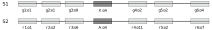
\includegraphics[width=\textwidth]{neighborhood.pdf}
  \caption{An illustration of the neighborhood similarity in terms of
    Orthogroups. Two neighborhoods of species $S1$ and $S2$ (top and
    bottom, respectively) have been     drawn. Genes in $S1$ are
    characterized with the letter {\bf g}, whereas in species $S2$ with
    the letter {\bf r}. The two focal genes are represented with the
    letter {\bf X} and {\bf A}, respectively. Orthogroups are denoted with the letter {\bf
      o}. Thus, {\bf g1:o1} represents the gene 1 in species $S1$
    which belongs to orthogroup 1. The two species, together, consist
    of 7 ({\bf o1}, {\bf o2}, {\bf o4}, {\bf o6}, {\bf o7}, {\bf o9}
    and {\bf o11})
    orthogroups. Out of them, 3 orthogroups ({\bf o1}, {\bf o2}, {\bf
      o4}) belong to both neighborhoods. Thus, the percent of
    similarity is $3/7 \approx 42.8\%$ }
  \label{fig:nei}
\end{figure}

\section*{Results}

A correlation example between human and cat

\begin{figure}[htbp!]
  \centering
  \includegraphics[width=\textwidth]{correlationPlot.pdf}
  \caption{The relation between {\it Homo sapiens} and {\bf Felis
      catus} regarding the orthogroup similarity of neighborhoods and
    percentage of alignment identity between two orthologous
    genes. The regression coefficient value is positive (15.873) and
    highly significant (pvalue $<10^{-16}$) illustrating that
    orthologous genes that are in similar neighborhoods (in terms of
    orthogroups) show less differences between them.}
  \label{fig:hcexample}
\end{figure}

\bibliographystyle{plainnat}
\bibliography{biblio}

\end{document}
